\chapter{Fiscal Policy (Text Ch. 29)}

\section{The federal budget}

\begin{definition}[Federal budget]
The \emph{federal budget} is the annual statement of the federal government's outlays
and revenues, together with the laws and regulations that approve and support them.
\end{definition}

The budget has two purposes:
\begin{enumerate}
  \item to finance the activities of the federal government; and
  \item to achieve macroeconomic objectives.
\end{enumerate}

\begin{definition}[Fiscal policy]
\emph{Fiscal policy} is the use of the federal budget to achieve macroeconomic objectives
such as full employment, sustained long-term economic growth and price level stability.
\end{definition}

\subsection{Budget making}

The federal government and Parliament make fiscal policy. After a long, drawn-out
process of consultations (with provinces, businesses and the public), the Minister of
Finance presents a budget to Parliament, usually in February or March; Parliament debates
and enacts the necessary legislation. Provincial and municipal governments have their own
budgets, and in Canada provincial spending is very large (health and education).

\subsection{Revenues and outlays}

\begin{itemize}
  \item \textbf{Revenues}: personal income taxes (the largest), corporate income taxes,
        indirect taxes (GST), and investment income.
  \item \textbf{Outlays}: transfer payments (to persons such as EI and Old Age Security,
        and to provinces such as the Canada Health Transfer and equalization),
        expenditure on goods and services, and debt interest.
\end{itemize}

\subsection{Budget balance}

\begin{definition}[Budget balance]
The government's \emph{budget balance} equals revenues minus outlays.
\begin{itemize}
  \item If revenues exceed outlays, the government has a \emph{budget surplus}.
  \item If outlays exceed revenues, it has a \emph{budget deficit}.
  \item If revenues equal outlays, it has a \emph{balanced budget}.
\end{itemize}
\end{definition}

\subsection{Deficit and debt}

\begin{definition}[Government debt]
\emph{Government debt} is the total amount that the government has borrowed. It equals the
sum of past deficits minus the sum of past surpluses. A deficit increases the debt; a
surplus decreases it.
\end{definition}

\begin{example}
Federal debt is \$600 billion. Over three years the government runs deficits of \$30 and
\$20 billion and then a surplus of \$10 billion. Debt becomes
$600 + 30 + 20 - 10 = \$640$ billion. If GDP grew from \$2{,}000 to \$2{,}200 billion
over the same period, the debt-to-GDP ratio fell from 30\% to about 29.1\%, even though
the debt rose.
\end{example}

\begin{remark}
Canada ran large deficits from the mid-1970s to the mid-1990s, followed by surpluses from
1997 to 2008 that cut the debt-to-GDP ratio sharply. Deficits returned after the 2008--2009
recession; in 2020--21 the COVID-19 response produced a federal deficit of over \$300
billion, the largest relative to GDP since the Second World War.
\end{remark}

\begin{important}[Pitfall: deficit vs debt]
The deficit is a \emph{flow} (per year); the debt is a \emph{stock} (accumulated).
Eliminating the deficit stops the debt from growing; it does not reduce the debt.
\end{important}

\section{Supply-side effects of fiscal policy}

Fiscal policy has important effects on employment, potential GDP and aggregate supply,
called \emph{supply-side effects}. They work through incentives.

\subsection{Income taxes and the labour market}

An income tax weakens the incentive to work: it drives a wedge between the wage that
firms pay and the wage that workers take home.

\begin{definition}[Tax wedge]
The \emph{tax wedge} is the gap between the before-tax wage rate and the after-tax wage
rate. Income taxes and taxes on expenditure (GST/HST) both contribute, since workers care
about what their take-home pay can buy.
\end{definition}

The income tax decreases the supply of labour (in terms of the before-tax wage), so the
before-tax wage rises, the after-tax wage falls, and the equilibrium quantity of labour
employed decreases. When employment at full employment decreases, \emph{potential GDP
decreases}, and LRAS shifts leftward.

\begin{example}[Size of the wedge]
The before-tax wage is \$20 an hour, the income tax rate is 20\% and the sales tax is
13\%. Take-home pay is $20 \times 0.8 = \$16$, which buys goods worth
$16/1.13 \approx \$14.16$ at pre-tax prices. The total tax wedge is
$20 - 14.16 = \$5.84$, about 29\% of the before-tax wage.
\end{example}

\subsection{Taxes and the incentive to save and invest}

A tax on interest income weakens the incentive to save and drives a wedge between the
interest rate paid by borrowers and the rate received by lenders. Because the tax is
levied on \emph{nominal} interest, its effect on the real after-tax rate is magnified by
inflation.

\begin{example}
Nominal interest rate 8\%, inflation 4\%, tax rate on interest income 25\%. The real
before-tax rate is $8 - 4 = 4\%$. The tax takes $0.25 \times 8 = 2$ percentage points, so the
after-tax nominal rate is 6\% and the real after-tax rate is $6 - 4 = 2\%$. The tax takes
half of the real return (an effective 50\% tax rate on real interest). Lower saving
decreases the supply of loanable funds, raises the real interest rate and reduces
investment and growth.
\end{example}

\subsection{Tax revenues and the Laffer curve}

\begin{definition}[Laffer curve]
The \emph{Laffer curve} is the relationship between the tax rate and the amount of tax
revenue collected. At a zero tax rate revenue is zero; at a 100\% rate nobody works for
pay and revenue is again zero; revenue is maximized at some intermediate rate.
\end{definition}

\begin{center}
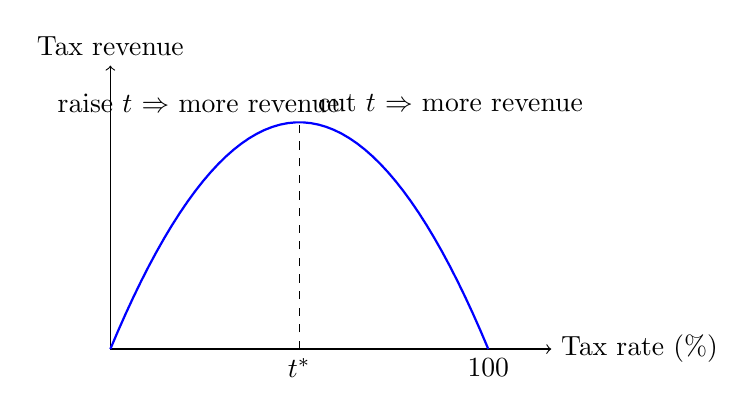
\begin{tikzpicture}[scale=0.8]
  \draw[->] (0,0) -- (7,0) node[right] {Tax rate (\%)};
  \draw[->] (0,0) -- (0,4.5) node[above] {Tax revenue};
  \draw[thick, blue, domain=0:6, samples=50] plot (\x, {0.4*\x*(6-\x)});
  \draw[dashed] (3,0) node[below] {$t^{*}$} -- (3,3.6);
  \node[below] at (6,0) {100};
  \node at (1.4,3.9) {raise $t$ $\Rightarrow$ more revenue};
  \node at (5.4,3.9) {cut $t$ $\Rightarrow$ more revenue};
\end{tikzpicture}
\end{center}

Below $t^{*}$, raising the tax rate raises revenue; above $t^{*}$, cutting the tax rate
\emph{raises} revenue because the tax base expands. Most evidence suggests Canada's
personal income tax rates are below the revenue-maximizing rate, so tax cuts reduce
revenue (but may still increase potential GDP).

\subsection{Generational effects}

Fiscal policy redistributes between generations: a deficit today must be paid for by
future taxpayers (or by cuts in future spending). \emph{Generational accounting} measures
the lifetime tax burden of each generation; a \emph{generational imbalance} exists when
future generations are expected to pay more than current ones. Public pensions (CPP, OAS)
financed by current workers are the main source.

\section{Fiscal stimulus}

\begin{definition}[Fiscal stimulus]
\emph{Fiscal stimulus} is the use of fiscal policy to increase production and employment.
It can be
\begin{enumerate}
  \item \textbf{automatic}: a fiscal policy action triggered by the state of the economy
        with no action by the government; or
  \item \textbf{discretionary}: a fiscal policy action initiated by an act of Parliament
        (a change in tax rates or a new spending program).
\end{enumerate}
\end{definition}

\subsection{Automatic fiscal policy and cyclical and structural balances}

Two features of the budget act as \emph{automatic stabilizers}:
\begin{itemize}
  \item \textbf{induced taxes}: tax revenues rise with real GDP, so in a recession taxes
        fall automatically, cushioning disposable income;
  \item \textbf{needs-tested spending}: transfer payments such as EI benefits and social
        assistance rise when unemployment rises.
\end{itemize}
Both make the budget move toward deficit in recessions and toward surplus in expansions,
which dampens fluctuations in AD (and also reduces the multiplier).

\begin{definition}[Structural and cyclical balance]
The \emph{structural surplus or deficit} is the budget balance that would occur if the
economy were at full employment (real GDP $=$ potential GDP). The \emph{cyclical surplus
or deficit} is the actual balance minus the structural balance; it arises purely from the
business cycle.
\end{definition}

\begin{example}
In a recession the actual federal deficit is \$30 billion. Estimates show that at full
employment the deficit would be \$10 billion (the structural deficit). The cyclical deficit
is $30 - 10 = \$20$ billion; it will disappear as the economy recovers, but the structural
deficit requires a policy change to eliminate.
\end{example}

\subsection{Discretionary fiscal stimulus: the fiscal multipliers}

Consider the simple Keynesian model with lump-sum taxes $T$, transfers, no income tax and
no imports, with marginal propensity to consume $b$. Then $C = a + b(Y - T)$ and
$Y = C + I + G$.

\begin{theorem}[Fiscal multipliers]
\begin{align*}
  \text{government expenditure multiplier} &= \frac{\Delta Y}{\Delta G} = \frac{1}{1 - b},\\
  \text{tax multiplier} &= \frac{\Delta Y}{\Delta T} = \frac{-b}{1 - b},\\
  \text{transfer payments multiplier} &= \frac{b}{1 - b},\\
  \text{balanced budget multiplier} &= \frac{1}{1 - b} + \frac{-b}{1 - b} = 1.
\end{align*}
\end{theorem}

\begin{proof}
Equilibrium: $Y = a + b(Y - T) + I + G$, so
\[
  Y = \frac{a - bT + I + G}{1 - b}.
\]
Differentiating with respect to $G$ gives $1/(1 - b)$; with respect to $T$ gives
$-b/(1 - b)$. A tax cut works only through consumption, and the first round of spending is
$b\,\Delta T$, not $\Delta T$ (part of the tax cut is saved), so the tax multiplier is
smaller in magnitude than the expenditure multiplier. A transfer is a negative tax. A
balanced budget change ($\Delta G = \Delta T$) adds the two effects to get 1.
\end{proof}

\begin{example}[Closing a recessionary gap]
Let $b = 0.75$. The expenditure multiplier is 4, the tax multiplier is $-3$ and the
balanced budget multiplier is 1. Real GDP is \$200 billion below potential (at a fixed
price level). To close the gap the government can
\begin{itemize}
  \item increase $G$ by $200/4 = \$50$ billion; or
  \item cut taxes by $200/3 \approx \$66.7$ billion; or
  \item increase $G$ and $T$ together by \$200 billion (balanced budget).
\end{itemize}
\end{example}

In the AS--AD model, fiscal stimulus shifts AD rightward by the multiplier times the
initial change. Because SRAS slopes upward, part of the effect raises the price level, so
real GDP increases by less than the fixed-price multiplier predicts. Fiscal stimulus can
also have \emph{supply-side} effects: a tax cut that raises the incentive to work also
increases potential GDP.

\subsection{Limitations of discretionary fiscal policy}

\begin{itemize}
  \item \textbf{Time lags}: the \emph{recognition lag} (time to recognize that action is
        needed), the \emph{law-making lag} (Parliament takes time to pass a budget), and
        the \emph{impact lag} (time for the change to affect real GDP). By the time it
        works, the economy may already have recovered.
  \item \textbf{Estimating potential GDP}: it is hard to tell whether a slowdown is
        cyclical or a fall in potential GDP; stimulus when real GDP is at potential creates
        inflation.
  \item \textbf{Crowding out}: deficit-financed stimulus raises the real interest rate and
        decreases private investment (see the loanable funds model).
  \item \textbf{Ricardo--Barro effect}: if people save a tax cut in anticipation of future
        taxes, the tax multiplier is close to zero.
  \item \textbf{Size of the multipliers}: with income taxes and imports (Canada imports
        about 30\% of GDP), real-world multipliers are much smaller than $1/(1 - b)$, and
        economists disagree about their size.
\end{itemize}

\section{Summary}

\begin{itemize}
  \item The federal budget finances government and is the instrument of fiscal policy.
        Budget balance $=$ revenues $-$ outlays; debt is accumulated past deficits minus
        surpluses (stock vs flow).
  \item Supply-side effects: income and expenditure taxes create a tax wedge that lowers
        employment and potential GDP; taxes on nominal interest income discourage saving
        (worse with inflation); the Laffer curve relates tax rates to revenue.
  \item Fiscal stimulus is automatic (induced taxes, needs-tested spending) or
        discretionary. Actual balance $=$ structural $+$ cyclical.
  \item Multipliers (simple model): $G$: $1/(1 - b)$; taxes: $-b/(1 - b)$; transfers:
        $b/(1 - b)$; balanced budget: 1.
  \item Discretionary policy faces time lags, uncertainty about potential GDP, crowding out
        and possibly the Ricardo--Barro effect.
\end{itemize}
